\section{Descrizione e motivazioni delle tecnologie adottate }
In questa sezione vengono presentate le tecnologie adottate per l’implementazione delle componenti client e server del sistema.
Inoltre, vengono descritte le architetture specifiche utilizzate nel back-end, in relazione alle tecnologie impiegate, e quelle adottate nel front-end.

\subsection{Tecnologie e architettura beckend}
L'architettura del nostro server è stata progettata per rispondere alle esigenze richieste dal cliente, dove è stata prioritizzata la velocità di sviluppo e deployment senza sacrificare robustezza e sicurezza. Abbiamo adottato un'architettura \textbf{monolitica} basata su una struttura a livelli, che facilita la separazione delle responsabilità e garantisce una maggiore manutenibilità nel tempo. La scelta di un'architettura monolitica si giustifica con la necessità di ridurre la complessità iniziale e non rallentare lo sviluppo, mantenendo comunque una struttura modulare che potrà essere facilmente evoluta nel tempo, ad esempio, trasformando parti del sistema in microservizi qualora il progetto dovesse espandersi in futuro.
\\
Le tecnologie selezionate per lo sviluppo del backend sono state scelte in base a una combinazione di familiarità e facilità d'uso, con l'obiettivo di accelerare il processo di implementazione e garantire al contempo solidità e qualità del codice.
\\
Il back-end è stato sviluppato utilizzando \textbf{Spring Boot}, abbiamo optato per questo framework grazie alle sue numerose configurazioni predefinite e utili estensioni come \textbf{Lombok}, che ci permettono di concentrarci sulla logica di business anziché su complesse configurazioni di sistema o codice ripetuto. Spring Boot consente di avviare rapidamente un'applicazione web robusta e scalabile.
esso sono state integrate diverse tecnologie complementari, tra cui:

\begin{itemize}
	\item \textbf{Hibernate}: Per la gestione della persistenza, Hibernate si rivela una scelta efficace, in quanto astrae le operazioni di accesso al database e riduce significativamente il lavoro manuale nella scrittura di query SQL. Questo approccio rende il codice più leggibile e facilmente mantenibile.
	
	\item \textbf{Spring Security e JWT (JSON Web Token)}: Per garantire un'autenticazione stateless e sicura, abbiamo deciso di utilizzare i JWT. Questa soluzione permette di gestire le sessioni degli utenti in maniera efficiente, differenziando eventuali ruoli o permessi e riducendo il carico sul server.
	
	\item \textbf{Jackson}: È uno strumento potente per serializzare e deserializzare oggetti Java in \textbf{JSON} e viceversa.
	Quando si utilizza l’annotazione \colorbox{lightgray}{@RestController} o \colorbox{lightgray}{@ResponseBody}, Spring Boot restituisce automaticamente le risposte in formato JSON senza necessità di configurazioni aggiuntive.
	
	\item \textbf{Swagger}: L’adozione di Swagger per la documentazione delle REST API agevola notevolmente il testing e la verifica degli endpoint, creando al contempo una documentazione ricca di informazioni utili per condividere informazioni critiche.
\end{itemize}

Il back-end del sistema segue il pattern architetturale \textbf{MVC (Model-View-Controller)}, nativamente supportato dal framework \textbf{Spring Boot}.
Nel nostro caso, il \textbf{Model} è rappresentato dalle entità e dalla logica di business implementata nei servizi; il \textbf{Controller} è costituito dai componenti RESTful che gestiscono e mappano le richieste HTTP.
La \textbf{View} non è gestita all’interno del back-end, poiché l’applicazione svolge il ruolo di \textbf{API REST}, restituendo risposte in formato JSON al client, che si occupa della rappresentazione dei dati.
Questo approccio garantisce una chiara \textbf{separazione delle responsabilità}, migliorando la \textbf{modularità} e la \textbf{manutenibilità} del sistema.
\\ \\
Di seguito viene riportato uno schema del design utilizzato del backend

\begin{figure}[H]
	\centering
	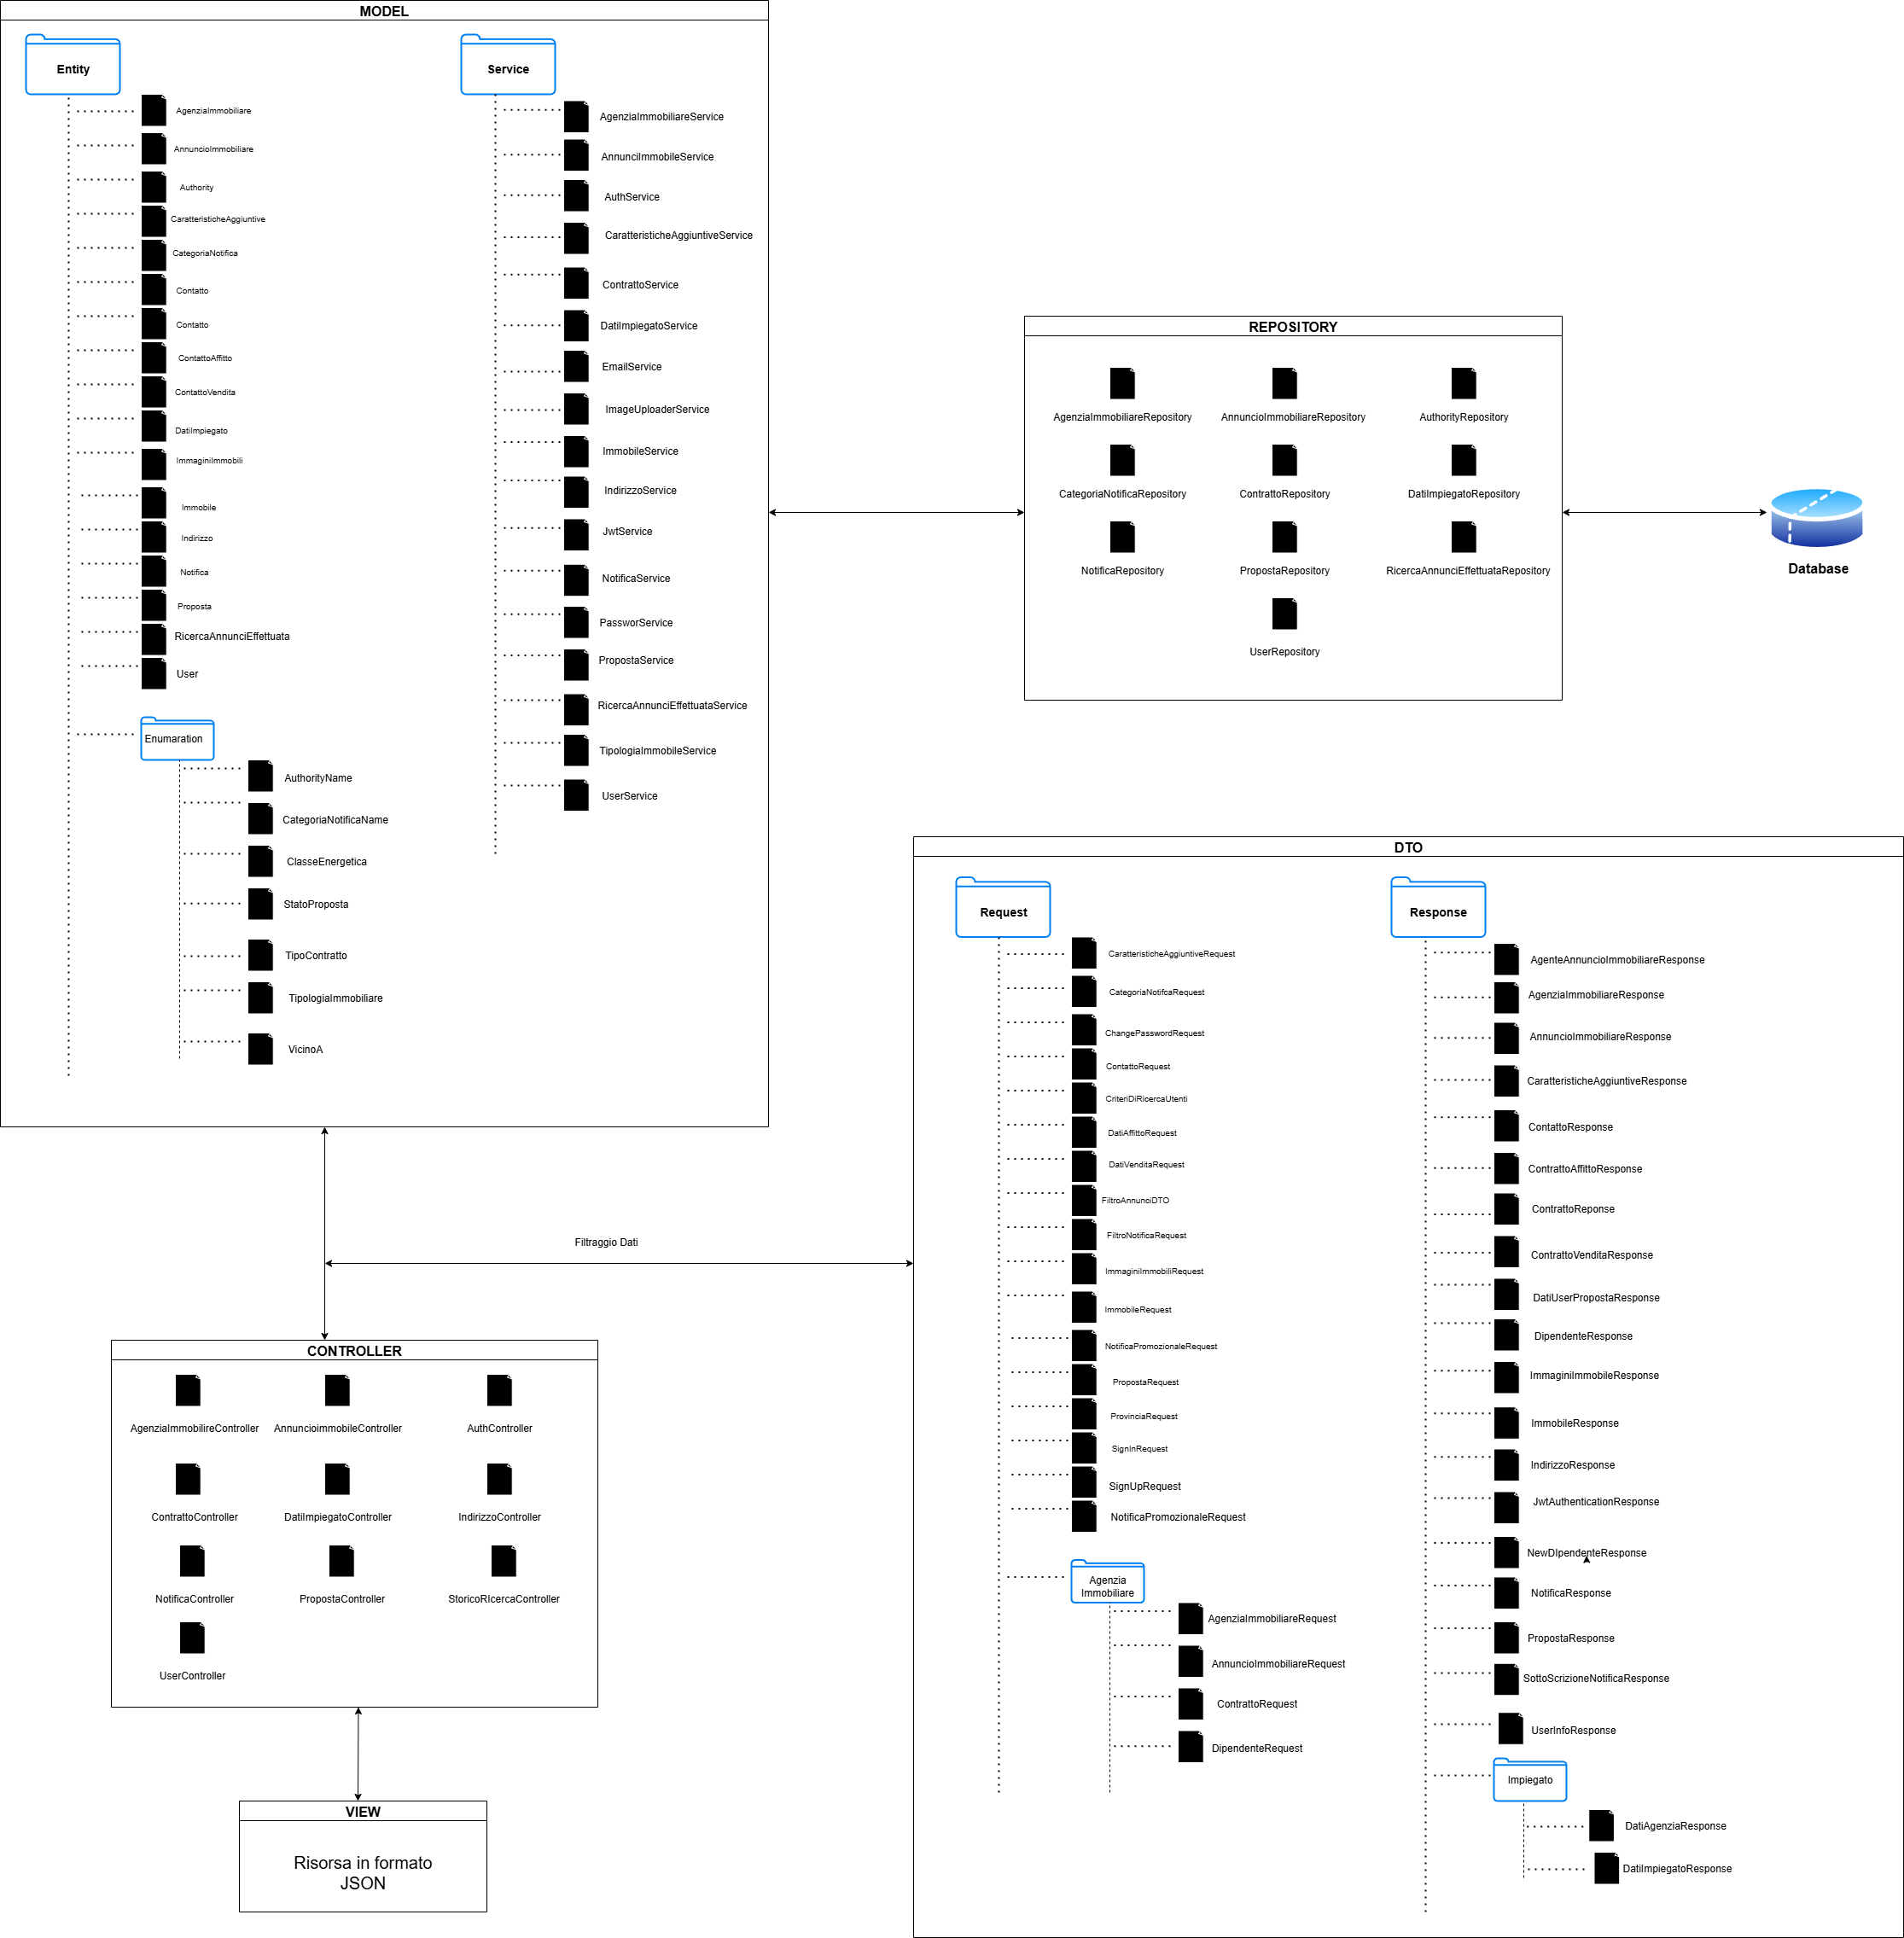
\includegraphics[width=0.7\linewidth]{Immagini/Schema backend.png}
	\caption[schema backend]{Schema sintetico dell'architettura del backend}
\end{figure}
